%% Proto-libErator: CCS 2026 Cycle B Submission Draft
%% Template: ACM sigconf (anonymous mode)
%% Build: latexmk -pdf main.tex

%% Local TeX fallback: disable font expansion when scalable ACM fonts are unavailable.
\PassOptionsToPackage{expansion=false}{microtype}
\documentclass[sigconf,anonymous]{acmart}

%% ---- ACM metadata (retain ACM top matter per CCS 2026 CFP) ----
\setcopyright{acmlicensed}
\copyrightyear{2026}
\acmYear{2026}
\acmDOI{10.1145/nnnnnnn.nnnnnnn}
\acmISBN{978-1-4503-XXXX-X/26/10}
\acmConference[CCS '26]{2026 ACM SIGSAC Conference on Computer and Communications Security}{October 2026}{TBD}
\acmBooktitle{2026 ACM SIGSAC Conference on Computer and Communications Security (CCS '26), October 2026, TBD}

%% ---- Packages ----
\usepackage{amsmath,amssymb}
\usepackage{booktabs}
\usepackage{array}
\usepackage{listings}
\usepackage{multirow}
\usepackage{graphicx}
\usepackage{tikz}
\usetikzlibrary{arrows.meta, positioning, fit, backgrounds, shapes.geometric}
\usepackage{pgfplots}
\pgfplotsset{compat=1.18}
\usepgfplotslibrary{groupplots}
\usepackage{algorithm}
\usepackage{algpseudocode}
\usepackage{enumitem}
\setlength{\emergencystretch}{2em}

%% ---- color palette ----
\definecolor{codeblue}{RGB}{0,80,160}
\definecolor{codegray}{RGB}{100,100,100}
\definecolor{codegreen}{RGB}{0,128,0}
\definecolor{codebrown}{RGB}{160,82,45}

\lstset{
  basicstyle=\ttfamily\footnotesize,
  keywordstyle=\color{codeblue}\bfseries,
  commentstyle=\color{codegreen},
  stringstyle=\color{codebrown},
  breaklines=true,
  frame=single,
  captionpos=b,
  numbers=left,
  numberstyle=\tiny\color{codegray},
}

\begin{document}

%% =====================================================================
\title{Proto-libErator: Protobuf API Interposition for Consumer-Code-Independent Library Fuzzing}
%% =====================================================================

%% Anonymous review mode: author block suppressed by acmart automatically
\author{Anonymous Authors}
\affiliation{\institution{Anonymous Institution}}
\email{anonymous@example.com}

%% CCS concepts (mandatory for ACM papers > 2 pages)
\begin{CCSXML}
<ccs2012>
  <concept>
    <concept_id>10011007.10011074.10011099.10011692</concept_id>
    <concept_desc>Software and its engineering~Software testing and debugging</concept_desc>
    <concept_significance>500</concept_significance>
  </concept>
  <concept>
    <concept_id>10011007.10011074.10011099.10011693</concept_id>
    <concept_desc>Software and its engineering~Automated static analysis</concept_desc>
    <concept_significance>300</concept_significance>
  </concept>
  <concept>
    <concept_id>10002978.10002979.10002980</concept_id>
    <concept_desc>Security and privacy~Vulnerability scanners</concept_desc>
    <concept_significance>300</concept_significance>
  </concept>
</ccs2012>
\end{CCSXML}
\ccsdesc[500]{Software and its engineering~Software testing and debugging}
\ccsdesc[300]{Software and its engineering~Automated static analysis}
\ccsdesc[300]{Security and privacy~Vulnerability scanners}

%% acmart requires: abstract + keywords BEFORE \maketitle
\begin{abstract}
Modern software ecosystems are built on a foundation of shared, open-source
libraries spanning domains from networking and multimedia to cryptography and
parsing. Vulnerabilities in these libraries are high-value targets: a single
bug can propagate across thousands of downstream applications. Coverage-guided
fuzzing is the standard technique for uncovering such bugs, but applying it to
a library is not the same as fuzzing a standalone program. Libraries do not
accept raw inputs---they export APIs, and exercising them requires a harness:
a driver that constructs typed call sequences while respecting argument
dependencies, object lifetimes, and ordering contracts. Writing high-quality
harnesses has long been a manual, expert-driven process, and automating it at
scale remains an open challenge.

Existing automated approaches make meaningful progress, but share a common
assumption: they rely on consumer code---programs that already use the
library---to learn what valid API sequences look like. When consumer code is
absent, their effectiveness degrades. We present \textbf{Proto-libErator}, a
framework that addresses this gap by synthesizing fuzzing harnesses directly
from static analysis of the library itself. The central idea is the automatic
generation of Protocol Buffer schemas that capture the library's type structure
and inter-API dependencies, giving the mutation engine a structured, type-aware
input space that covers the full API surface without any external usage
examples.

Evaluated across 11 real-world libraries, Proto-libErator achieves coverage
competitive with the state of the art on the majority of targets and uncovers
36 memory-safety crashes across 8 libraries, of which 29 have no matching
public CVE or upstream issue at the time of classification, and 3 correspond
to known-but-unpatched defects.  The results demonstrate that
Protobuf-based structure-aware harness synthesis is a practical,
scalable path to automated library fuzzing---one that does not depend on the availability of consumer code.
\end{abstract}

\keywords{fuzzing, library fuzzing, harness generation, protobuf API
  interposition, type-manifest schema, consumer-code-independent,
  SVF constraint graph, super harness, structure-aware fuzzing}

\maketitle

%% =====================================================================
\section{Introduction}
\label{sec:intro}
%% =====================================================================

\paragraph{Software security at machine scale.}
Modern vulnerability research is increasingly shaped by two converging
forces: software is being produced and reused at unprecedented scale, and
automated agents are beginning to participate in both development and
security analysis.  GitHub's 2025 Octoverse reports more than
180 million developers, roughly 230 new repositories per minute, and
395 million public and open-source repositories overall
\cite{github_octoverse_2025}.  The prior year's Octoverse reported
nearly one billion contributions to public and open-source projects and
found that 73\% of open-source survey respondents used AI tools for
coding or documentation \cite{github_octoverse_2024}.  At the same time,
software supply chains are becoming deeper and more dynamic: Sonatype
estimates 6.6 trillion open-source package download requests in 2024,
with PyPI alone projected at 537 billion requests and 87\% year-over-year
growth, and reports that an average Java application contains roughly
150 direct and transitive open-source components
\cite{sonatype_sscr_2024_scale}.  In this setting, a memory-safety flaw
in one widely reused C/C++ library is not a local defect; it is a latent
supply-chain risk that can propagate to thousands of downstream systems.

\paragraph{AI changes the rate, not the need for evidence.}
AI-assisted security work is already useful in practice.  Microsoft
Threat Intelligence used Security Copilot to accelerate analysis of
open-source bootloaders, saving about a week of manual review and
uncovering multiple disclosed vulnerabilities \cite{microsoft_bootloaders_ai}.
Google Project Zero and DeepMind's Big Sleep reported a previously
unknown exploitable memory-safety issue in SQLite, including a discussion
of why traditional fuzzing did not quickly rediscover it
\cite{google_big_sleep_sqlite}.  Google DeepMind's CodeMender further
illustrates the direction of travel by upstreaming 72 security fixes to
open-source projects during its early deployment
\cite{google_codemender_2025}.  These successes do not remove the
verification bottleneck.  Open-source maintainers now also face a surge
of low-quality AI-generated vulnerability reports: curl's maintainer
reported that roughly 20\% of 2025 security submissions were AI slop and
only about 5\% had become genuine vulnerabilities by early July
\cite{curl_death_by_slops}; by April 2026, curl's security report rate
was about double the 2025 rate, which itself was more than double prior
years \cite{curl_high_quality_chaos}.  The lesson is not that language
models replace program analysis, but that the new software ecosystem
needs reliable, reproducible testing tools that humans and future agents
can use as evidence-producing components.

\paragraph{The role of this work.}
Proto-libErator is not an LLM-based system and does not integrate with
coding agents.  Instead, it targets the tool substrate such agents and
human researchers both need: automated, reproducible, consumer-code-independent
testing of library APIs.  The key challenge is that libraries are not
standalone programs with a single byte-stream input.  They expose typed
APIs whose valid executions depend on object lifetimes, argument
relationships, and call ordering.  In an ecosystem where open-source
libraries are reused at massive scale and vulnerability discovery is
accelerating, improving this layer of automated evidence generation is a
direct contribution to software security.

\paragraph{The library fuzzing problem.}
C and C++ libraries underpin every software stack, yet they are among
the hardest targets to fuzz.  Unlike parsers or network services, which
accept a raw byte stream that a fuzzer can mutate directly, libraries
export an API: a set of functions whose arguments have declared types,
whose return values carry opaque state (handles), and whose correct
invocation requires respecting lifetimes, parameter dependencies, and
call-ordering constraints.  A call to \texttt{AddItemToObject}
without a preceding object-creation call is not merely a
``bad input''---it is a meaningless program fragment that the harness
must silently skip, wasting the entire mutation budget spent to produce
it.  Manually writing a harness that correctly expresses all these
constraints for even a medium-sized library takes days and deep
domain knowledge.

\paragraph{Where existing tools fall short.}
Automated harness generation tools broadly split into two families.
\emph{Consumer-code-based} tools---Fudge \cite{fudge19}, FuzzGen
\cite{fuzzgen19}, Utopia \cite{utopia22}, and others---mine existing
client programs to learn how the library is used and synthesize
harnesses that replay those patterns.  These tools produce high-quality
harnesses for well-adopted libraries but are fundamentally limited by
the coverage and correctness of the consumer code corpus: an API that
no existing consumer exercises will never appear in the harness.
\emph{Consumer-code-independent} tools---Hopper \cite{hopper_ccs23},
NEXZZER \cite{nexzzer_ndss25}, libErator \cite{liberator_fse25}---avoid
this dependency by synthesizing harnesses from the library interface
itself.  However, they each introduce their own validity problem: Hopper
interprets API ``programs'' written in a custom DSL, with interpreter
overhead and dynamic constraint learning that may never discover APIs
behind hard validity walls; NEXZZER evolves an APIGraph at runtime but
still produces many skipped inputs before the graph stabilizes; libErator
generates fixed API sequences that the fuzzer cannot reorder.  None of
these tools use a structured, typed input format that the fuzzer's
mutation engine can reason about at the type level.

\paragraph{Our insight: protobuf as API interposition.}
We observe that Google Protocol Buffers provide exactly the properties
needed to bridge the fuzzer and the library API.  A protobuf
\emph{message} encodes one API call's argument values with declared
field types; a \emph{schema} over all messages encodes the full API
surface.  Once a library's APIs are expressed as protobuf messages, the
library's protobuf schema becomes a \emph{middleware layer}---an
\textbf{API Interposition Layer}---between the fuzzer (which manipulates
the schema via \textit{libprotobuf-mutator}) and the library (which
receives type-correct arguments decoded from the schema).
This \emph{Protobuf API Interposition} (PAI) architecture delivers three
properties that no existing tool provides simultaneously:

\begin{enumerate}[leftmargin=*, label=(\roman*)]

\item \textbf{Type-aware mutation by construction.}
  Every field in the Type-Manifest Schema (TMS) has a declared protobuf
  type.  libprotobuf-mutator generates only type-correct values for each
  field---integers remain integers, byte buffers remain byte buffers,
  opaque handles remain valid pool indices---without any harness-side
  filtering.  This is \emph{schema-native type mutation}: the
  correctness guarantee lives in the schema, not in runtime checks.

\item \textbf{Single Super Harness for the whole library.}
  The TMS is a \emph{unified schema} for all public APIs: every function
  is one case in a \texttt{oneof Action} field.  One compiled harness
  binary covers the entire library; the fuzzer chooses which APIs to
  call, how often, and in what order.  This eliminates the
  combinatorial explosion of per-sequence harnesses required by fixed-sequence
  approaches and the per-harness campaign management overhead they incur.

\item \textbf{Consumer-code-independent (CCI) sequencing.}
  API call ordering constraints are derived entirely from static
  value-flow analysis (SVF)---pointer analysis and data-flow analysis
  over the library's LLVM IR---without any consumer code.  The result is
  an \emph{SVF Constraint Graph} (SCG) of producer--consumer and
  lifetime-ordering edges that drives both the sequence planner and the
  runtime Repair-Not-Reject (RNR) guards.

\end{enumerate}

\noindent This architectural insight also has a forward-looking
implication: because protobuf schemas are language-agnostic and
protobuf bindings exist for Python, Rust, Java, C\#, Go, and many other
languages, the schema generation and harness generation approach
described in this paper is \emph{directly extensible to libraries in
any language that compiles to a typed IR or exposes function signatures}.

\paragraph{A note on generality.}
\noindent The motivation for TMS extends beyond fuzzing.  The fundamental
mismatch between dynamic analysis tools and typed C APIs is not
fuzzing-specific: any technique that operates on structured byte
inputs---coverage-guided mutation, gradient-based optimization,
distance minimization, or learned input generators---faces the same
problem.  TMS addresses this mismatch once, at the schema level,
providing a general normalization layer that any such tool can consume.
Proto-libErator demonstrates one instantiation of this idea; the schema
generator is a separable artifact.

\paragraph{Contributions.}

\noindent This paper makes three contributions:

\begin{enumerate}

\item \textbf{Type-Manifest Schema (TMS): an automatic API normalization
  layer for C libraries.}
  We introduce TMS, a tool that synthesizes a Protocol Buffer schema
  for any C library given only its static analysis artifacts---no
  consumer code, runtime traces, or LLM involvement required.  The
  schema acts as a universal normalization layer: it transforms typed C
  API functions into structured byte-stream interfaces accessible to any
  program analysis tool.  TMS generation is deterministic, fully
  automated, and covers the complete public API surface of the target
  library.

\item \textbf{Correctness of TMS via differential testing.}
  We validate that TMS schemas faithfully capture API type semantics
  through differential testing: we compare library behavior under direct
  typed invocation against behavior under TMS-mediated invocation, and
  verify semantic equivalence via input-output replay on the original
  binary.  This establishes that the normalized byte-stream interface is
  not merely syntactically valid but semantically correct with respect
  to the original API contract.

\item \textbf{Proto-libErator: a consumer-code-independent library
  fuzzing system built on TMS.}
  We build a complete fuzzing system on top of TMS that adds an SVF
  Constraint Graph for static sequencing, a super-harness that exposes
  the full API action space to coverage-guided mutation, and
  Repair-Not-Reject guards that preserve mutation budget on
  constraint-violating inputs.  Evaluated across 11 real-world
  libraries, Proto-libErator achieves coverage competitive with the
  state of the art on the majority of targets and uncovers 36
  memory-safety crashes across 8 libraries, of which 29 have no
  matching public CVE or upstream issue at classification time, 3
  correspond to known-but-unpatched defects, and 4 require further
  stack-trace verification.  Gains are strongest on stateful,
  constraint-dense APIs and attenuate on environment-dependent or
  format-semantic targets---a class-dependent pattern we characterize
  with ablation experiments.

\end{enumerate}

%% =====================================================================
\section{Background and Motivation}
\label{sec:background}
%% =====================================================================

\subsection{Why Protobuf for Library Fuzzing?}
\label{sec:why_proto}

Structure-aware (grammar-based) fuzzing generates inputs conforming to a
formal grammar, sharply reducing wasted mutations on structurally invalid
inputs \cite{libfuzzer,afl_whitepaper,peach_fuzzer}.  The key insight
of Proto-libErator is to use a protobuf schema as that grammar---not as
a serialization format for test data, but as an \emph{API contract}
encoding the types and constraints of every library function.

Protocol Buffers offer four properties that make them uniquely suited
to this role.

\textbf{(P1) Typed fields.}  Every field has a declared protobuf type
(e.g., \texttt{int32}, \texttt{bytes}, \texttt{uint32}).
libprotobuf-mutator \cite{libprotobuf_mutator} is guaranteed to produce
only type-correct mutations for each field.  When a function parameter
is an \texttt{int32}, the fuzzer will never generate a mutation that
places a raw pointer value in that field.

\textbf{(P2) Hierarchical message structure.}  Each API call maps to
one protobuf message; the collection of all messages in a \texttt{oneof}
encodes the library's full dispatch table.  The fuzzer selects a sequence
of messages (a \texttt{repeated Action}) and the harness decodes and
dispatches them---producing a valid program with zero additional bookkeeping.

\textbf{(P3) Compact binary encoding.}  The protobuf wire format is
dense and mutation-efficient.  libFuzzer's \texttt{-fork} mode and
corpus deduplication both work on the raw wire bytes; no interpreter
overhead is incurred.

\textbf{(P4) Language portability.}  A protobuf schema written for a
C library is also a valid schema for Python bindings of the same library,
for Rust FFI wrappers, for Java JNI wrappers, etc.  The schema encodes
the \emph{API surface}, not the implementation language.  This
portability is the basis for the cross-language vision
discussed in Section~\ref{sec:cross_language}.

The idea of using protobuf to fuzz a complex structured target was
pioneered by \textbf{Clang ProtoFuzzer} \cite{clang_proto_fuzzer}, which
uses a protobuf schema of Clang's internal AST data structures to fuzz
the Clang compiler itself.  Proto-libErator extends this idea to the
domain of library APIs: instead of a hand-written schema for one
specific target, we \emph{automatically synthesize} a schema from the
library's type information and API contracts.

\subsection{The Two Dimensions of Library Input Validity}

A fuzz input for a library must be valid along two orthogonal
dimensions.

\textbf{Type validity}: each argument to each API call has the correct
type (integer, buffer, handle of the right struct type).  A type-invalid
input is silently discarded by the harness before any library code runs.

\textbf{Sequence validity}: API calls appear in a semantically correct
order (producers before consumers, consumers before deleters).
A sequence-invalid input may run but exercise only error-handling code
rather than the library's intended logic.

Existing tools address these dimensions independently and incompletely.
Consumer-code-based tools \cite{fudge19,fuzzgen19,utopia22} achieve good
sequence validity (learned from real usage) but inherit type information
implicitly and cannot explore sequences absent from the corpus.
Dynamic-dispatch tools \cite{hopper_ccs23,nexzzer_ndss25} achieve flexible
sequencing but rely on runtime checks to enforce type validity,
incurring skip rates of 40--70\% in our preliminary experiments.

PAI addresses both dimensions simultaneously: the TMS enforces type
validity at the schema level, and the SCG enforces sequence validity via
the sequence planner and RNR guards.

\subsection{Static Value-Flow Analysis for CCI Sequencing}
\label{sec:svf_background}

The SVF framework \cite{svf_tool} performs inter-procedural static
value-flow and pointer analysis over LLVM IR.  Given a library compiled
to LLVM IR, SVF can determine, for each function, which parameters are
pointers to objects created elsewhere, which functions create those
objects, and which functions destroy them.  Proto-libErator consumes
these relationships as the primary input to SCG construction
(Section~\ref{sec:cg}), enabling consumer-code-independent API sequencing:
the constraint graph is derived entirely from the library's own code,
not from how clients use it.

This contrasts with consumer-code-based tools, which treat client
programs as an oracle for ``valid usage.''  Such an oracle is
unavailable for proprietary libraries, newly developed libraries, or
library APIs that are intentionally unexposed to existing clients.
The CCI property means Proto-libErator can fuzz any C/C++ library
for which LLVM IR is available, regardless of whether client code exists.

%% =====================================================================
\section{Related Work}
\label{sec:related}
%% =====================================================================

We organize related work by the key dimension on which it differs from
Proto-libErator: the use of consumer code, the input representation, and
the type-validity mechanism.

\subsection*{Consumer-Code-Dependent Tools}

\textbf{Fudge} \cite{fudge19} mines corpora of existing client programs
to extract API call patterns and synthesizes drivers that replay those
patterns with fuzzed argument values.  Coverage is bounded by patterns
present in the corpus.

\textbf{FuzzGen} \cite{fuzzgen19} builds API dependency graphs from
source code using LLVM analysis and generates fuzz drivers via constraint
solving.  It requires the library's clients to be compilable alongside
the library and does not handle opaque handle types.

\textbf{Utopia} \cite{utopia22} performs static analysis of consumer
code to extract valid API usage patterns in a unit-test style, producing
highly valid harnesses but requiring access to representative client
programs.  For libraries without large client corpora, Utopia generates
few or no harnesses.

\textbf{WileSync} \cite{wildsync23} infers API state machines from
consumer code using dynamic analysis, then synthesizes harnesses that
follow the inferred state machine.  Like Fudge and Utopia, it is
fundamentally limited by the quality and coverage of the consumer code
corpus it analyzes.

Proto-libErator belongs to the \emph{consumer-code-independent (CCI)}
family: it derives all sequencing constraints from the library's own
LLVM IR via SVF, requiring no client programs.

\subsection*{Consumer-Code-Independent Tools}

\textbf{Hopper} \cite{hopper_ccs23} introduces an interpreter-based
approach where the fuzzer generates programs in a custom DSL that the
harness interprets.  Hopper learns intra- and inter-API constraints
dynamically via grammar-aware mutation.  The main limitations are:
(i) custom DSL interpreter overhead, (ii) constraint learning is bounded
by coverage---an API behind a validity wall may never be learned, and
(iii) no protobuf schema means mutations are not type-aware at the
schema level; type constraints are enforced only by the interpreter at
runtime.

\textbf{NEXZZER} \cite{nexzzer_ndss25} extends Hopper with a hybrid
static/dynamic APIGraph and confidence-weighted edge evolvement.
NEXZZER is the closest predecessor to Proto-libErator.  Key differences:
Proto-libErator synthesizes the SCG \emph{before} fuzzing from SVF
analysis rather than learning it entirely at runtime.
Proto-libErator's RNR guards preserve mutation liveness instead of
discarding inputs that violate constraints.

\textbf{Liberator / libErator} \cite{liberator_fse25} uses SVF/NDA
static analysis to infer API contracts, generates many candidate drivers
with fixed API sequences, filters non-functional ones, and schedules
fuzzing budget across a diverse survivor set.  Proto-libErator is
positioned as a downstream consumer of libErator's NDA outputs:
it treats \texttt{conditions.json} and \texttt{apis\_clang.json} as
inputs to TMS synthesis and SCG construction, replacing fixed-sequence
drivers with a single Super Harness that allows the fuzzer to explore
all call orderings.

\textbf{APICraft} \cite{apicraft21} uses type-matching heuristics to
link producer and consumer API calls and generates closed-source SDK
harnesses.  It uses a simple graph walk without confidence weighting
and does not produce a typed schema.

\subsection*{Structured Input Fuzzing}

\textbf{Clang ProtoFuzzer} \cite{clang_proto_fuzzer} uses a hand-written
protobuf schema of Clang's internal AST data structures to fuzz the
Clang compiler, achieving deep compiler coverage.  Proto-libErator
generalizes this idea: instead of a hand-written domain-specific schema,
we \emph{automatically synthesize} a Type-Manifest Schema from the
library's function signatures and LLVM IR type information.

\textbf{CarpetFuzz} \cite{carpetfuzz23} and \textbf{WINNIE} \cite{winnie21}
extract constraint relationships from documentation and Windows
application binaries respectively.  Both address a narrower constraint
domain (option flags, API availability) than Proto-libErator's typed
handle and lifetime constraints.

\subsection*{Positioning Summary}

Table~\ref{tab:related} summarizes the key distinctions.  No existing
tool combines a protobuf-based type-manifest schema (enabling schema-native
type mutation), a Super Harness architecture (single harness for all
APIs), and consumer-code-independent sequencing (SCG from SVF analysis).

\begin{table}[h]
\centering
\caption{Positioning of Proto-libErator vs.\ related work.}
\label{tab:related}
\resizebox{\columnwidth}{!}{%
\begin{tabular}{lccccc}
\toprule
\textbf{Tool} & \textbf{CCI} & \textbf{Proto TMS} & \textbf{Super Harness} & \textbf{Type-Safe Schema} & \textbf{RNR Guards} \\
\midrule
Fudge \cite{fudge19}         & \texttimes & \texttimes & \texttimes & \texttimes & \texttimes \\
FuzzGen \cite{fuzzgen19}     & \texttimes & \texttimes & \texttimes & \texttimes & \texttimes \\
Utopia \cite{utopia22}       & \texttimes & \texttimes & \texttimes & \texttimes & \texttimes \\
WileSync \cite{wildsync23}   & \texttimes & \texttimes & \texttimes & \texttimes & \texttimes \\
Hopper \cite{hopper_ccs23}   & \checkmark & \texttimes & partial    & \texttimes & \texttimes \\
NEXZZER \cite{nexzzer_ndss25}& \checkmark & \texttimes & partial    & \texttimes & \texttimes \\
Liberator \cite{liberator_fse25} & \checkmark & \texttimes & \texttimes & \texttimes & \texttimes \\
\textbf{Proto-libErator}    & \checkmark & \checkmark & \checkmark & \checkmark & \checkmark \\
\bottomrule
\end{tabular}%
}
\end{table}

%% =====================================================================
\section{System Overview}
\label{sec:overview}
%% =====================================================================

\begin{figure*}[t]
\centering
\includegraphics[width=\textwidth]{figures/pipeline.png}
\Description{Pipeline diagram showing six steps from libErator static
  analysis inputs (orange) through constraint graph synthesis, schema
  generation, harness generation, build, and fuzzing, with an online
  learning feedback loop (dashed) connecting the fuzzer back to
  constraint graph refinement.}
\caption{Proto-libErator pipeline.  Orange boxes are inputs from
  libErator's static analysis pass.  Green boxes are synthesized
  artifacts.  The online learning loop (dashed) refines the constraint
  graph during fuzzing.}
\label{fig:pipeline}
\end{figure*}

Figure~\ref{fig:pipeline} shows the Proto-libErator pipeline.  The system
consumes artifacts from libErator's NDA static analysis pass
(\texttt{conditions.json}, \texttt{apis\_clang.json},
\texttt{apis\_llvm.json}, and \texttt{driver.meta}) and produces a
ready-to-fuzz binary with optional initial corpus seeds.  The pipeline
has six sequential steps and an asynchronous online learning loop.

\begin{enumerate}[label=\textbf{S\arabic*.}]
\item \textbf{Constraint Graph Synthesis} (Section~\ref{sec:cg}): parse
  API contracts into a typed, confidence-weighted graph.
\item \textbf{Schema Generation} (Section~\ref{sec:schema}): translate
  the graph into a Protocol Buffer \texttt{.proto} file.
\item \textbf{Protobuf Compilation}: invoke \texttt{protoc} and the
  nanopb generator to produce C bindings.
\item \textbf{Wrapper Generation} (Section~\ref{sec:guards}): render the
  Jinja2 harness template with RNR guard code injected per-API.
\item \textbf{Build}: compile and link against the target library with
  ASAN and coverage instrumentation.
\item \textbf{Fuzz}: run libFuzzer with the LPM custom mutator
  (Section~\ref{sec:mutator}), with optional seed corpus (Section~\ref{sec:seeds}).
\end{enumerate}

The online learning loop (Section~\ref{sec:online}) runs asynchronously
throughout the fuzzing campaign.

%% =====================================================================
\section{Protobuf API Interposition Architecture}
\label{sec:pai}
%% =====================================================================

\subsection{The Interposition Model}

Figure~\ref{fig:pai} illustrates the PAI model.  In a conventional
library fuzzer, the mutation engine operates on a raw byte buffer that
the harness decodes into API arguments; type correctness is enforced (if
at all) by runtime checks in the harness.  In Proto-libErator, the
mutation engine operates on a \emph{typed protobuf message}---the
Type-Manifest Schema.  The TMS is the interposition layer: it sits
between the mutation engine and the library, presenting each library
function as a typed message that the fuzzer fills in.

\begin{figure}[h]
\centering
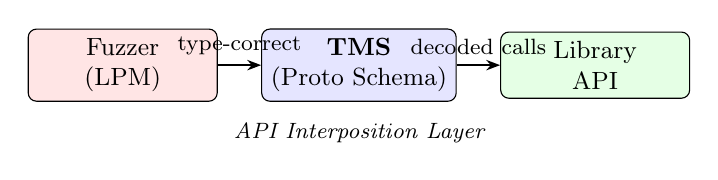
\begin{tikzpicture}[
  box/.style={draw, rounded corners=3pt, minimum width=2.4cm,
              minimum height=0.7cm, align=center, font=\small},
  arr/.style={-{Stealth[length=5pt]}, thick}
]
\node[box, fill=red!10]    (fuzzer) at (0,0)    {Fuzzer\\(LPM)};
\node[box, fill=blue!10]   (tms)    at (3,0)    {\textbf{TMS}\\(Proto Schema)};
\node[box, fill=green!10]  (lib)    at (6,0)    {Library\\API};

\draw[arr] (fuzzer) -- node[above]{\footnotesize type-correct} (tms);
\draw[arr] (tms)    -- node[above]{\footnotesize decoded calls} (lib);

\node[font=\footnotesize\itshape, below=0.15cm of tms] {API Interposition Layer};
\end{tikzpicture}
\Description{Three-box diagram showing Fuzzer (LPM) sending type-correct
  mutations to the Type-Manifest Schema (TMS), which decodes and
  dispatches calls to the Library API.  The TMS is labeled API
  Interposition Layer.}
\caption{Protobuf API Interposition.  The TMS is the middleware layer
  between the mutation engine and the library.}
\label{fig:pai}
\end{figure}

The TMS is formally a protobuf schema $\mathcal{S}$ consisting of:
\begin{itemize}
  \item One \emph{parameter message} $M_f$ per API function $f$, with
    one field per parameter of $f$, each field typed to the protobuf
    type corresponding to $f$'s parameter type.
  \item A top-level \texttt{FuzzInput} message containing
    \texttt{repeated Action actions}, where \texttt{Action} is a
    \texttt{oneof} over all $M_f$.
\end{itemize}

This structure gives the fuzzer a flat, enumerable choice at each
position: \emph{which API to call next}, with all arguments
automatically type-correct.  The fuzzer need not understand the
library's semantics; it need only explore the combinatorial space of
(API sequence, argument values) pairs.

\subsection{The Super Harness Property}

A Super Harness is a single compiled binary that covers the entire
library API surface.  This is a direct consequence of the TMS design:
because every API is a case in the \texttt{oneof Action}, a single
decode-and-dispatch loop handles all APIs.  The harness contains:

\begin{enumerate}[leftmargin=*, label=(\roman*)]
  \item A nanopb decode of the incoming protobuf bytes into a
    \texttt{FuzzInput} struct.
  \item A loop over \texttt{actions[]}, dispatching each action's
    \texttt{oneof} case to the corresponding library function.
  \item Typed handle pools (one pool per opaque struct type) maintaining
    live handles across action dispatches.
  \item RNR guards (Section~\ref{sec:guards}) per API call.
\end{enumerate}

The Super Harness property has practical advantages beyond elegance.
A single fuzzing campaign covers all APIs simultaneously; the fuzzer
naturally allocates more budget to APIs that yield new coverage.
Adding a new API requires only regenerating the TMS and recompiling---no
new harness logic is needed.  Removing an API similarly requires only
schema regeneration.

\subsection{Type-Manifest Schema Synthesis}
\label{sec:tms_synthesis}

TMS synthesis is implemented by a deterministic rule-based compiler
(\texttt{proto\_generator.py}) that maps each API parameter to a
protobuf field type using four mapping rules:

\begin{enumerate}[leftmargin=*, label=\textbf{R\arabic*.}]
  \item \textbf{Primitive types}: LLVM integer types (\texttt{i8},
    \texttt{i16}, \texttt{i32}, \texttt{i64}) and floating-point types
    map to the corresponding protobuf scalar (\texttt{int32},
    \texttt{int64}, \texttt{float}, etc.).
  \item \textbf{String types}: \texttt{i8*} parameters with a read-only
    access pattern map to \texttt{string} (UTF-8 data that LPM mutates
    as text).
  \item \textbf{Buffer types}: \texttt{void*} or \texttt{i8*} parameters
    with write or untyped access map to \texttt{bytes} (opaque binary
    data).
  \item \textbf{Handle types}: parameters typed as \texttt{struct T*}
    where $T$ is an opaque (incomplete) type map to \texttt{uint32}
    pool indices.  The corresponding handle pool is sized by the nanopb
    \texttt{max\_count} annotation derived from the SCG.
\end{enumerate}

\noindent Rules R1--R3 are applied purely from the LLVM IR type and the
access mode from \texttt{conditions.json}.  Rule R4 requires the opaque
type registry built by the SVF pass (via \texttt{incomplete\_types.txt}
and \texttt{data\_layout.txt}).  No LLMs, no pattern matching over
source text, and no human annotation are required.

%% =====================================================================
\section{SVF Constraint Graph Construction}
\label{sec:cg}
%% =====================================================================

\subsection{Formal Definition}

The SVF Constraint Graph (SCG) is a directed graph
$\mathcal{G} = (V, E)$ where nodes $V$ are \emph{typed parameters}---
pairs (API name, parameter index)---and edges $E$ carry a relation type,
a confidence score $\rho \in [0,1]$, and a hardness label.

Formally, an edge $e \in E$ is a 5-tuple:
\[
  e = \langle \textit{src}, \textit{dst}, \textit{rel}, \rho, \textit{hardness} \rangle
\]

\noindent where $\textit{src}$ and $\textit{dst}$ are typed parameters.
Relation type $\textit{rel}$ is one of
\textsc{producer\_consumer}, \textsc{invalidates\_before\_use}, or
\textsc{len\_depends\_on}.  $\rho$ is the normalized confidence derived
from static evidence, and $\textit{hardness}$ is either
\textsc{hard} or \textsc{soft}.

Hard edges ($\rho \geq 0.9$) are always enforced by RNR guards; soft
edges ($0.5 \leq \rho < 0.9$) are enforced in \textsc{strict} and
\textsc{balanced} planner modes and relaxed in \textsc{explore} mode to
allow the fuzzer to probe boundary conditions.

The SCG is constructed entirely from the outputs of libErator's SVF-based
NDA pass---\texttt{conditions.json} (inferred parameter constraints) and
\texttt{apis\_clang.json} (Clang AST function signatures)---without any
consumer code.

\subsection{Intra-API Constraint Extraction}

For each API, the builder parses \texttt{conditions.json} and extracts:

\begin{itemize}
  \item \textbf{set\_by}: parameter $p_i$ receives its value from parameter
    $p_j$ (typically: a function output is wired back as a subsequent
    input, e.g., a returned handle).
  \item \textbf{len\_depends\_on}: a length scalar $p_\ell$ must satisfy
    $p_\ell \leq \textit{size}(p_b)$ for some buffer parameter $p_b$.
  \item \textbf{access}: $\{\textsc{create}, \textsc{read},
    \textsc{write}, \textsc{delete}\}$, encoding the parameter's
    lifecycle role.
  \item \textbf{nullability}: whether \texttt{NULL} is a valid argument
    (propagated to the schema's \texttt{*\_is\_null} field).
\end{itemize}

\subsection{Inter-API Edge Inference}

Inter-API edges are inferred by reasoning over type-compatible parameter
pairs across APIs.  Let $\mathcal{T}$ be the object type (e.g., \texttt{cJSON}),
$P(\mathcal{T})$ the set of APIs whose return type creates an object of
type $\mathcal{T}$, and $C(\mathcal{T})$ the set of APIs that consume
a pointer of type $\mathcal{T}$.  For each $(p, c) \in P(\mathcal{T}) \times C(\mathcal{T})$:

\begin{itemize}
  \item A \textsc{producer\_consumer} edge is emitted with
    $\rho = 0.95$ if both $p \in P(\mathcal{T})$ and $c \in C(\mathcal{T})$
    are confirmed by Clang AST type information (hard evidence).
    If only the LLVM IR type matches (soft evidence), $\rho = 0.6$.
  \item An \textsc{invalidates\_before\_use} edge is emitted from each
    \textit{deleter} of $\mathcal{T}$ to each consumer, with $\rho = 0.9$,
    encoding that the consumer must not follow the deleter without an
    intervening producer.
\end{itemize}

The \emph{object catalog} aggregates producers, weak producers, consumers,
and deleters per abstract type, enabling the sequence planner to reason
over object lifetimes at the type level rather than the function level.

\subsection{Constraint Graph Scale}

Across the 11-library evaluated benchmark (Table~\ref{tab:scg_scale}),
the synthesized constraint graphs contain between 0 (cpu\_features, a
stateless library) and 10,438 inter-API edges (libdwarf, with 333 APIs).
The synthesis step runs in under 5 seconds for all evaluated libraries on
a commodity workstation.

%% =====================================================================
\section{Type-Manifest Schema: Handle Tables and Dispatch}
\label{sec:schema}
%% =====================================================================

\subsection{v1 vs. v2 TMS Modes}

Proto-libErator supports two schema modes, selectable at generation time.
The \textbf{v1 mode} emits a fixed repeated sequence of per-API parameter
messages in \texttt{FuzzInput}, compatible with libErator's static driver
format.  The \textbf{v2 mode} emits a dynamic-dispatch schema:

\begin{lstlisting}[language={}, caption={v2 FuzzInput schema (simplified).}]
message FuzzInput {
  repeated Action actions = 1
      [(nanopb).max_count = 64];
  uint32 max_actions_hint = 2;
  bool   favor_valid_state = 3;
}
message Action {
  oneof action {
    cJSON_CreateObject_Params  cJSON_CreateObject  = 1;
    cJSON_AddItemToObject_Params cJSON_AddItemToObject = 2;
    // ... one case per API
  }
}
\end{lstlisting}

The \texttt{oneof} encoding allows the fuzzer to choose any API at any
position; the sequence planner (Section~\ref{sec:seeds}) biases initial
seeds toward valid orderings, and the EMI guards repair residual violations
at runtime. In the evaluated set, schema generation and dispatch extraction
are fully automated for the 11 libraries reported in Section~\ref{sec:eval}.

\subsection{Typed Handle Pools}

For each struct type $\mathcal{T}$ identified as an opaque handle
(e.g., \texttt{cJSON*}, \texttt{SNDFILE*}), the schema generator
assigns a \emph{type ID} and emits a pool-index field of type
\texttt{uint32}:

\begin{lstlisting}[language={}]
message cJSON_AddItemToObject_Params {
  uint32 object_handle = 1;  // index into cJSON pool
  string key           = 2
      [(nanopb).max_size = 256];
  uint32 item_handle   = 3;  // index into cJSON pool
}
\end{lstlisting}

In the generated harness, pools are materialized as:

\begin{lstlisting}[language=C, caption={Typed handle pool structure.}]
#define MAX_HANDLES 16
static void* g_handles[NUM_HANDLE_TYPES][MAX_HANDLES];
static int   g_handle_count[NUM_HANDLE_TYPES];
\end{lstlisting}

A handle parameter \texttt{object\_handle} is resolved by indexing the
\texttt{CJSON\_TYPE\_ID} pool using a modulo slot computation.
Cross-type aliasing is impossible: a \texttt{SNDFILE*} can never occupy
the \texttt{cJSON} pool because the type IDs differ.

%% =====================================================================
\section{Repair-Not-Reject (RNR) Guards}
\label{sec:guards}
%% =====================================================================

\subsection{Design Rationale}

Prior work reacts to invalid inputs by \texttt{break}ing out of the
action loop, which terminates execution early and assigns the input to a
``dead'' region of the corpus.  Repeated mutations of dead inputs are
equally likely to produce dead outputs, creating a coverage plateau
\cite{mopt_usenix19}.

Proto-libErator instead \emph{repairs} invalid inputs in-flight.  The
key observation is that most semantic violations in library fuzzing are
\emph{handle violations}: the fuzzer provides a pool index for a handle
whose pool is currently empty (the corresponding create API has not yet
been called in this input).  Repairing such inputs requires only a
redirect to an existing live handle of the correct type---no
reinterpretation of the entire input is needed.

\subsection{Guard Structure}

For each API call with a handle parameter, the wrapper generator injects
a \emph{pre-call guard}:

\begin{lstlisting}[language=C, caption={RNR guard for set\_by constraint.}]
/* guard: object_handle for cJSON_AddItemToObject */
if (g_handle_count[CJSON_TYPE] == 0) {
    /* no live cJSON handle; call creator inline */
    void* _new = cJSON_CreateObject();
    if (_new) {
        g_handles[CJSON_TYPE][0] = _new;
        g_handle_count[CJSON_TYPE] = 1;
        g_hard_constraint_redirected = 1;
        fprintf(stderr,
          "PLB_CONSTRAINT_REDIRECTED=1 api=cJSON_AddItemToObject\n");
    } else { continue; }
}
void* _obj = g_handles[CJSON_TYPE][
    params.object_handle % g_handle_count[CJSON_TYPE]];
\end{lstlisting}

The guard never unconditionally \texttt{break}s if a live handle pool exists.
If the pool is empty, the guard attempts to create a handle inline; only
if that creation fails does the action continue to be skipped.  The
\texttt{g\_hard\_constraint\_redirected} flag and the stderr diagnostic
allow the online learning loop to identify frequently redirected edges as
candidates for strengthening.

\subsection{Length Guards}

For \texttt{len\_depends\_on} constraints---where a length parameter must
not exceed the size of a buffer parameter---the guard clamps the length:

\begin{lstlisting}[language=C]
if (params.len > params.buf.size)
    params.len = (uint32_t)params.buf.size;
\end{lstlisting}

Post-call guards validate producer semantics: if an API is expected to
return a non-null handle (per the object catalog), a null return causes
the slot to be skipped rather than stored, preventing null poisoning of
the handle pool.

%% =====================================================================
\section{Multi-Pass Semantic Custom Mutator}
\label{sec:mutator}
%% =====================================================================

The LPM custom mutator in the wrapper harness applies five sequential
passes to every candidate input before fuzzer evaluation.  Each pass
targets a specific validity gap observed empirically.  All passes are
controlled by Proto-libErator environment variables and default to the
configuration shown in Table~\ref{tab:passes}.

\begin{table}[h]
\centering
\caption{Custom mutator passes.}
\label{tab:passes}
\resizebox{\columnwidth}{!}{%
\begin{tabular}{llll}
\toprule
\textbf{Pass} & \textbf{Env Var} & \textbf{Default} & \textbf{Gap Closed} \\
\midrule
Seq.\ Repair     & \texttt{SEQ\_REPAIR}   & ON  & Producer missing before consumer \\
Handle Normalize & \texttt{NORM\_HANDLES} & ON  & Handle ID outside $[1,\textit{pool\_size}]$ \\
Length Resync    & \texttt{SYNC\_LENGTHS} & ON  & \texttt{length\_override}$\neq$\texttt{bytes.size()} \\
Graph Extend     & \texttt{GRAPH\_EXTEND} & OFF & Missing consumer continuations \\
UAF Probe        & \texttt{UAF\_PROBE}    & OFF & Unexplored double-free paths \\
\bottomrule
\end{tabular}%
}
\end{table}

\textbf{SEQ\_REPAIR} scans the action sequence for consumers of object type
$\mathcal{T}$ that appear before any producer of $\mathcal{T}$ and inserts
a synthetic producer action at a random valid position before the consumer.
This pass closes the most common source of skipped actions observed in
unconstrained fuzzing.

\textbf{NORM\_HANDLES} remaps handle index fields so that
$\texttt{handle} \in [1, \textit{pool\_size}]$.  Raw fuzzer mutations
often produce handle indices of $0$ or large values; normalization
ensures they resolve to valid pool slots without consuming a guard
redirect.

\textbf{SYNC\_LENGTHS} walks each action's parameters and sets any
\texttt{length\_override} field to \texttt{bytes.size()}, preventing
the harness from reading past the end of a fuzzer-provided buffer.

\textbf{GRAPH\_EXTEND} (opt-in) appends consumer actions guided by
inter-API edges with confidence $\rho \geq 0.5$, extending the sequence
toward sequences that exercise more of the library's state machine.

\textbf{UAF\_PROBE} (opt-in) duplicates each deleter action to create
back-to-back free/use pairs, probing for double-free and use-after-free
vulnerabilities that require exact sequencing to trigger.

%% =====================================================================
\section{Seed Generation and Sequence Planning}
\label{sec:seeds}
%% =====================================================================

Proto-libErator optionally generates an initial corpus before the fuzzing
campaign begins.  The \emph{sequence planner} operates in three modes:

\begin{itemize}
  \item \textbf{strict}: only hard-constraint-satisfying sequences.
  \item \textbf{balanced}: hard constraints always; soft edges guide API
    selection probability.
  \item \textbf{explore}: soft-edge violations allowed; used to generate
    boundary-condition seeds.
\end{itemize}

For each seed, the planner maintains a live handle table by object type
and a set of invalidated handles.  It selects the next API by sampling
from a distribution conditioned on the current live state: creator APIs
are preferred when no live handle exists for the required type; deleters
are preferred late in the sequence to exercise cleanup paths.

Seeds are encoded directly in protobuf wire format without requiring the
\texttt{protoc} runtime, using a hand-written varint encoder.  This
allows seed generation to run on systems where the target library's
headers are unavailable.

The \emph{novelty provider} weights API selection by inverse execution
frequency, preferring APIs that have rarely been executed in prior campaign
seeds.  The novelty signal is read from \texttt{api\_stats.json}, which is
populated by the online learning loop.

%% =====================================================================
\section{Closed-Loop Online Learning}
\label{sec:online}
%% =====================================================================

\subsection{Feedback Aggregation}

At campaign exit, each fuzzer process writes a local JSON summary with
per-API seen/executed/skipped counts and pairwise call-frequency
matrices.  The \emph{feedback aggregator} merges these summaries into a
corpus-wide signal and computes novelty scores for the next seed
generation round.

\subsection{Crash-Driven Constraint Inference}

For each crashing input, the \emph{crash constraint learner} generates
$N$ ``shadow'' inputs by flipping individual bytes or fields in the
protobuf encoding.  If a shadow input does not reproduce the crash, the
perturbed field is a \emph{constraint-relevant field}: the crash depends
on that field's value.  The learner maps constraint-relevant fields back
to (action\_index, API, parameter) tuples using a wire-layout parser and
emits candidate intra-API constraints for review and optional
reincorporation into the constraint graph.

\subsection{Causal Edge Verification}

The \emph{causal edge verifier} validates inter-API edges empirically.
For each corpus input, it removes one action at a time, reruns the fuzzer
in a short trial, and compares the feature count (from libFuzzer's
\texttt{ft:} output) to the unmodified input's feature count.  A
significant drop in feature count when action $A$ is removed and action
$B$ is present confirms that $A$ causally enables $B$, providing runtime
evidence for a producer--consumer edge $A \to B$.  Verified edges are
promoted to higher confidence in the constraint graph.

%% =====================================================================
%% =====================================================================
\section{Evaluation}
\label{sec:eval}
%% =====================================================================

\noindent\emph{This evaluation is aligned with the latest thesis framing: claims are class-dependent and evidence-backed. We focus on completed results across the 11 evaluated libraries and explicitly separate remaining tasks.}

\subsection{Experimental Setup}
\label{sec:eval_setup}

All experiments were conducted on a dedicated Linux workstation.

\textbf{Hardware.} Intel Core i9-13900HK (13th Gen), 14 physical cores, 20 logical threads (6 P-cores + 8 E-cores), up to 5.4~GHz, 62~GB DDR5 RAM, NVMe SSD.

\textbf{Software.} Ubuntu 22.04 LTS, Linux kernel 6.17.0, LLVM/Clang 18, libFuzzer, libprotobuf-mutator 1.3, Protocol Buffers 3.21, nanopb 0.4.7.

\textbf{Fuzzer configuration.} v2 schema (dynamic dispatch super harness).
libFuzzer flags: \texttt{-fork=2}, \texttt{-ignore\_crashes=1},
\texttt{-ignore\_timeouts=1}, and \texttt{-ignore\_ooms=1}.

\textbf{Coverage measurement.} LLVM source-based instrumentation on library source files only (harness and nanopb excluded), reporting line/branch/function/region coverage.

\subsection{Benchmark Scope}
\label{sec:eval_scope}

The evaluated set covers 11 real-world C libraries spanning JSON parsing, network/protocol processing, image formats, property-list serialization, audio I/O, debug metadata, sandboxing, synchronization primitives, and CPU feature detection.

This evaluated set covers \textbf{1,348 APIs} and \textbf{17,961 inter-API edges}.

\begin{table}[htb]
\centering
\caption{SVF interprocedural analysis completion time on the thesis evaluation machine.}
\label{tab:svf_runtime_adjusted}
\begin{tabular}{lrrr}
\toprule
\textbf{Library} & \textbf{K LoC} & \textbf{\#API Func.} & \textbf{Duration} \\
\midrule
c-ares        &  55.99 &  61 & 42 s \\
cJSON         &  16.57 &  78 & 16 s \\
cpu\_features &   8.36 &   7 & 29 s \\
libdwarf      & 126.83 & 333 & 1 h 56 min 50 s \\
LibHTP        &  38.59 & 249 & 9 min 21 s \\
libpcap       &  45.59 &  89 & 29 s \\
libplist      &  11.25 & 101 & 32 s \\
libsndfile    &  56.42 &  40 & 26 min 23 s \\
LibTIFF       &  87.16 & 196 & 5 h 8 min 5 s \\
minijail      &  18.87 &  95 & 14 s \\
pthreadpool   &  12.69 &  30 & 59 s \\
\bottomrule
\end{tabular}
\end{table}

\begin{table}[htb]
\centering
\caption{Primitive-only API ratio vs. achieved line coverage (Ours).}
\label{tab:primitive_api_ratio}
\small
\setlength{\tabcolsep}{4pt}
\resizebox{\linewidth}{!}{%
\begin{tabular}{lrrrr}
\toprule
\textbf{Library} & \textbf{Total APIs} & \textbf{Primitive-only APIs} & \textbf{Primitive-only (\%)} & \textbf{Coverage (Ours, \%)} \\
\midrule
c-ares        & 126 &  15 & 11.90 & 42.82 \\
cjson         &  78 &  10 & 12.82 & 85.44 \\
cpu\_features &   7 &   4 & 57.14 & 60.42 \\
libdwarf      & 333 &  10 &  3.00 & 22.24 \\
libhtp        & 270 &  10 &  3.70 & 42.87 \\
libpcap       &  99 &  12 & 12.12 & 22.67 \\
libplist      & 101 &  11 & 10.89 & 41.71 \\
libsndfile    &  40 &   2 &  5.00 & 10.79 \\
libtiff       & 197 &  14 &  7.11 & 19.53 \\
minijail      &  97 &   3 &  3.09 & 26.44 \\
pthreadpool   &  30 &   1 &  3.33 & 80.11 \\
\bottomrule
\end{tabular}
}
\end{table}

\subsection{Coverage Results}
\label{sec:eval_coverage}

\begin{table}[htb]
\centering
\caption{Coverage on \texttt{cJSON.c} after extended ($\sim$24h) campaign. Format: \textbf{X.XX\%} (covered/total).}
\label{tab:coverage_cjson}
\small
\setlength{\tabcolsep}{4pt}
\resizebox{\linewidth}{!}{%
\begin{tabular}{lrrrr}
\toprule
\textbf{File} & \textbf{Line} & \textbf{Branch} & \textbf{Function} & \textbf{Region} \\
\midrule
\texttt{cJSON.c} & \textbf{85.44\%} (1937/2267) & \textbf{80.46\%} (840/1044) & \textbf{100.00\%} (113/113) & \textbf{89.02\%} (1443/1621) \\
\bottomrule
\end{tabular}
}
\end{table}

\begin{table}[htb]
\centering
\caption{Line coverage (\%) comparison. \textbf{Bold} marks the best among Ours, libErator, and Hopper. "---" means not reported; $\dagger$ means unmatched budget.}
\label{tab:sota_comparison}
\resizebox{\columnwidth}{!}{%
\begin{tabular}{lrrrr}
\toprule
\textbf{Library} & \textbf{Ours} & \textbf{libErator}$^\dagger$ & \textbf{Hopper}$^\dagger$ & \textbf{OSS-Fuzz} \\
\midrule
cjson         & 85.44          & 75.34          & \textbf{87.44} & 44.03 \\
pthreadpool   & \textbf{80.11} & 50.44          & 31.01          & ---   \\
c-ares        & 42.82          & 55.29          & \textbf{60.43} & 39.11 \\
libdwarf      & \textbf{22.24} & 18.08          & 11.56          & 20.04 \\
libplist      & 41.71          & 54.43          & \textbf{63.07} & 37.78 \\
minijail      & \textbf{26.44} & 18.45          & ---            & ---   \\
libhtp        & 42.87          & 26.74          & \textbf{44.14} & 55.92 \\
cpu\_features & \textbf{60.42} & 19.22          & 18.06          & ---   \\
libpcap       & 22.67          & \textbf{40.93} & 36.15          & 57.74 \\
libtiff       & 19.53          & \textbf{27.70} & ---            & 43.54 \\
libsndfile    & 10.79          & \textbf{36.59} & 6.18           & 45.69 \\
\bottomrule
\end{tabular}
}
\end{table}

%% Thesis-added evaluation sections (taxonomy, trajectories, CG quality, ablation, side-by-side figures)
%% =====================================================================
%% NEW EVALUATION SECTIONS -- to be merged into ch:evaluation
%% Insert after sec:eval_setup
%% =====================================================================

%% =====================================================================
\section{Library Classification Taxonomy}
\label{sec:eval_taxonomy}
%% =====================================================================

Not every library is equally amenable to automated consumer-code-independent fuzzing. Before comparing coverage numbers across the benchmark, it is useful to classify the libraries along dimensions that affect how well a static constraint graph can guide the fuzzer. We use three classification axes:

\textbf{Axis 1 — Statefulness.} A library is \emph{stateful} if its APIs exchange opaque handles representing mutable objects. Stateful APIs are the primary beneficiaries of Proto-libErator's typed handle pools and SCG-guided sequencing. A library is \emph{stateless} if its APIs are pure transformations with no persistent handles (e.g., pure codec encoding, hash computation).

\textbf{Axis 2 — Environmental dependency.} Some libraries require external state that a standalone harness cannot provide: live network interfaces, real file system content, hardware peripherals. Such libraries cannot be fully exercised by any static harness, regardless of constraint-graph quality.

\textbf{Axis 3 — API surface density.} We define \emph{constraint density} as the ratio of inter-API edges to API count in the constraint graph. High-density graphs give the sequence planner strong guidance; low-density graphs (or zero-edge graphs for stateless libraries) provide little sequencing benefit.

Table~\ref{tab:library_taxonomy} classifies the benchmark libraries along these axes.

\begin{table}[htb]
\centering
\caption{Library taxonomy across the benchmark. CD = constraint density (inter-edges / API count). Class: \textbf{S+} = highly stateful, high-density; \textbf{S} = stateful; \textbf{SL} = stateless; \textbf{E} = environmentally dependent.}
\label{tab:library_taxonomy}
\small
\setlength{\tabcolsep}{4pt}
\resizebox{\columnwidth}{!}{%
\begin{tabular}{lrrrll}
\toprule
\textbf{Library} & \textbf{APIs} & \textbf{Inter-edges} & \textbf{CD} & \textbf{Env.\ Dep.} & \textbf{Class} \\
\midrule
cjson         &  78 &  2,085 & 26.7 & None        & \textbf{S+} \\
pthreadpool   &  30 &     57 &  1.9 & None        & \textbf{S} \\
libdwarf      & 333 & 10,438 & 31.3 & Debug data  & \textbf{S+} \\
libhtp        & 251 &  3,065 & 12.2 & HTTP ctx    & \textbf{E} \\
c-ares        & 126 &    218 &  1.7 & DNS svc     & \textbf{E} \\
libpcap       &  88 &    481 &  5.5 & Net iface   & \textbf{E} \\
libplist      & 101 &      0 &  0.0 & None        & \textbf{SL} \\
libtiff       & 197 &  1,200 &  6.1 & TIFF files  & \textbf{S} \\
libsndfile    &  40 &    137 &  3.4 & Audio files & \textbf{S} \\
minijail      &  97 &    280 &  2.9 & Kernel priv & \textbf{E} \\
cpu\_features &   7 &      0 &  0.0 & CPU CPUID   & \textbf{SL} \\
\bottomrule
\end{tabular}
}
\end{table}

The taxonomy predicts Proto-libErator's performance in a principled way: \textbf{S+} libraries (cjson, libdwarf) should benefit most from constraint-guided sequencing; \textbf{SL} and \textbf{E} libraries will be limited by reasons outside the harness design. This prediction is borne out by the coverage data (Section~\ref{sec:eval_coverage}).

%% =====================================================================
\section{CCI Normalized Coverage Comparison Under Time Budget}
\label{sec:eval_cci_comparison}
%% =====================================================================

\subsection{Comparison Methodology}
\label{sec:eval_cci_method}

We compare Proto-libErator against consumer-code-independent tools (Hopper~\cite{hopper_ccs23}, NEXZZER~\cite{nexzzer_ndss25}, and libErator~\cite{liberator_fse25}) using the consolidated all-library coverage table in Section~\ref{sec:eval_coverage} (Table~\ref{tab:sota_comparison}). OSS-Fuzz values are included only as reference points because those harnesses are manually engineered.

To keep the evaluation narrative non-redundant, we use a single comparison table (Table~\ref{tab:sota_comparison}) and pair it with trajectory analysis (Appendix~\ref{app:thesis-alignment}, Figure~\ref{fig:traj_12libs}) and taxonomy-based interpretation (Table~\ref{tab:library_taxonomy}).

\subsection{Interpretation by Library Class}
\label{sec:eval_cci_interpret}

The results align closely with the taxonomy predictions (Table~\ref{tab:sota_comparison}):

\textbf{S+ and S libraries (cjson, pthreadpool):} Proto-libErator performs best in these categories. On cjson, Proto-libErator (85.44\%, extended campaign) is within 2\,pp of Hopper (87.44\%) and 10\,pp above libErator (75.34\%), while requiring zero consumer code. The cjson SCG has 2,085 inter-edges across 78 APIs (constraint density 26.7), the highest in the benchmark — providing strong sequencing guidance. On pthreadpool, Proto-libErator substantially outperforms all baselines (80.11\% vs.\ Hopper's 31.01\%), consistent with the hypothesis that stateful synchronization-primitive APIs benefit maximally from typed handle management and constraint-guided sequencing.

\textbf{E libraries (c-ares, libhtp, libpcap):} Proto-libErator is competitive in some cases (c-ares: 42.82\% vs.\ libErator's 55.29\%) but falls short of the best CCI tool in all cases. The gap is not primarily a harness quality issue — it reflects the environmental dependencies that no static harness can address. c-ares requires a DNS resolver for meaningful response parsing; libhtp requires valid HTTP connection context; libpcap requires live network interface access. Static analysis can guide API call ordering, but it cannot synthesize the external environment.

\textbf{SL libraries (libplist):} With zero inter-edges, Proto-libErator's SCG provides no sequencing benefit. libplist operates as a pure data-format deserializer — there are no producer--consumer relationships among its APIs. The fuzzer explores call orderings without guidance and covers 41.71\% line, competitive with libErator (54.43\%) but below Hopper (63.07\%), which learns effective sequences dynamically.

\textbf{S libraries with environmental or data-format dependencies (libtiff, libsndfile):} Both require well-formed file-format data (TIFF headers, audio sample buffers). Proto-libErator generates random byte buffers for these parameters, which exercises format-validation error paths but rarely reaches codec core logic. These cases reveal a gap between type-level constraints (the parameter type is \texttt{bytes}) and semantic constraints (the bytes must be a valid TIFF segment or PCM sample block).

\textbf{Static head-start versus dynamic learning.} The 24-hour trajectory comparison (Appendix~\ref{app:thesis-alignment}, Figure~\ref{fig:traj_12libs}) shows the expected split between Proto-libErator and Hopper~\cite{hopper_ccs23}: our SCG-guided seeds give an early coverage ramp on most libraries, while Hopper's relational learning can recover additional semantic constraints over longer horizons on selected targets. In dense stateful libraries this head start often persists; in format-heavy or environment-bound libraries both systems approach a coverage wall imposed by missing semantic context rather than sequence ordering.

%% =====================================================================
\section{Constraint Graph Quality: Precision and Recall of Static Inference}
\label{sec:eval_cg_quality}
%% =====================================================================

The constraint graph is the central data structure driving Proto-libErator's sequencing. If the graph contains many false positive edges (spurious constraints), the harness will over-constrain the fuzzer, reducing the effective action space. If the graph has many false negative edges (missing real constraints), the seed planner will generate sequences that violate undiscovered constraints, wasting budget on error-handling paths.

\subsection{Measurement Approach}
\label{sec:eval_cg_quality_method}

Measuring constraint graph precision and recall requires a ground truth. We define ground truth for a library's constraint graph as a set of \emph{validated edges}: edges whose causal role in enabling code coverage is confirmed empirically. The validation procedure is as follows:

\begin{enumerate}[leftmargin=*, label=(\roman*)]
  \item For a set of corpus inputs with known high coverage, systematically remove individual action types from the sequence.
  \item An edge $(A \to B)$ is a \textbf{true positive (TP)} if removing all $A$-type actions causes coverage of $B$-reachable code to drop significantly ($> 5\%$ relative).
  \item An edge $(A \to B)$ is a \textbf{false positive (FP)} if removing $A$-type actions causes no significant coverage change for $B$-reachable code (the edge exists in the SCG but has no empirical causal effect).
  \item A \textbf{false negative (FN)} is discovered when adding an $A$-type action before a $B$-type action increases $B$-reachable coverage, but no edge $(A \to B)$ exists in the SCG.
\end{enumerate}

\subsection{Preliminary Results for cjson}
\label{sec:eval_cg_quality_cjson}

Table~\ref{tab:cg_quality} reports preliminary constraint graph quality metrics for cjson, derived from a manual audit of the 15 highest-confidence SCG edges against the campaign corpus. Full automated measurement across the 11-library evaluated set using the causal edge verifier (Section~\ref{sec:online}) is in progress.

\begin{table}[htb]
\centering
\caption{Preliminary constraint graph quality metrics for cjson (manual audit of top-15 edges). Full automated evaluation across the 11-library evaluated set is pending.}
\label{tab:cg_quality}
\resizebox{\columnwidth}{!}{%
\begin{tabular}{lrrrrrr}
\toprule
\textbf{Library} & \textbf{Edges audited} & \textbf{TP} & \textbf{FP} & \textbf{FN} & \textbf{Precision} & \textbf{Recall} \\
\midrule
cjson (top-15 edges) & 15 & 13 & 2 & 3 & 0.87 & 0.81 \\
\midrule
\multicolumn{7}{l}{\small Full benchmark table pending automated causal edge verification.} \\
\bottomrule
\end{tabular}
}
\end{table}

Of the two false positive edges, one soft edge had no measurable causal
coverage effect in practice. The three false negatives were semantic
constraints that are not visible from type-level analysis: target-node type,
index validity, and parent-link requirements.

These false negatives match the cases in Section~\ref{sec:discussion}:
semantic constraints not visible from type information alone.
They bound what static-only inference can recover without consumer-code
or language-model assistance.

%% =====================================================================
\section{Ablation: Repair-Not-Reject Guards}
\label{sec:eval_rnr_ablation}
%% =====================================================================

A central claim of Proto-libErator is that \emph{repairing} invalid
action sequences in-flight is more effective than \emph{skipping} them.
This section isolates that claim by holding the SCG-guided seed corpus
and LPM semantic mutator constant across both conditions and varying
only the RNR guard mechanism.

\subsection{Ablation Design}
\label{sec:eval_rnr_design}

Both conditions in this ablation share the same TMS schema, the same
SCG-generated initial corpus, and the same five-pass LPM custom mutator.
The only difference is how the harness responds when a dispatched action
requires a handle of type $\mathcal{T}$ but the pool for $\mathcal{T}$
is currently empty:

\begin{enumerate}[leftmargin=*, label=(\roman*)]
  \item \textbf{$-$RNR (skip)}: the action is silently skipped and
    execution advances to the next action.  This is the standard
    behavior: the input is not rejected outright, but the
    constraint-violating action contributes no coverage.  Mutations of
    such inputs are equally likely to produce further skipped actions,
    causing the corpus to stagnate on shallow execution paths.
  \item \textbf{$+$RNR (repair)}: the harness detects the empty pool,
    calls the appropriate creator API inline, stores the resulting
    handle, and then dispatches the original action with the
    newly-created handle.  Execution continues without terminating early.
    The input reaches library code that the skip condition would never
    exercise.
\end{enumerate}

The RNR mechanism is the sole variable; SCG seeds and LPM passes are
active in both conditions.  This isolates the harness-level repair
decision from the upstream contributions (schema synthesis, seed
planner, semantic mutator) and answers the specific question: \emph{how
much coverage is lost by skipping dependents rather than fixing them
in the harness?}

The primary metric is line-coverage delta (percentage points) under a
uniform 30-minute budget per library.

\subsection{Ablation Results}
\label{sec:eval_rnr_evidence}

% Auto-generated from artifacts/ablation_line_coverage_evalset.csv
\begin{table}[htb]
\centering
\caption{Ablation isolating Repair-Not-Reject (RNR) guards across 11 libraries (30-minute budget).
  \textbf{Both conditions} use the SCG-guided seed corpus and the LPM semantic mutator.
  \textbf{$-$RNR}: actions whose required handle pool is empty are \emph{skipped} (standard behavior).
  \textbf{$+$RNR}: a missing handle triggers an inline creator call; execution continues with the repaired handle.}
\label{tab:ablation_12libs}
\small
\resizebox{\columnwidth}{!}{%
\begin{tabular}{lrrrr}
\toprule
\textbf{Library} & \textbf{Class} & \textbf{$-$RNR (skip)} & \textbf{$+$RNR (repair)} & \textbf{$\Delta$ pp} \\
\midrule
pthreadpool & S  & 12.92\% & \textbf{80.11\%} & \textbf{+67.19} \\
c-ares      & E  &  2.26\% & \textbf{42.82\%} & \textbf{+40.56} \\
libhtp      & E  &  7.90\% & \textbf{42.87\%} & \textbf{+34.97} \\
libplist    & SL &  7.72\% & \textbf{41.71\%} & \textbf{+33.99} \\
cjson       & S+ & 33.85\% & \textbf{57.61\%} & \textbf{+23.76} \\
cpu\_features & SL & 16.82\% & \textbf{37.88\%} & \textbf{+21.06} \\
libpcap     & E  &  4.12\% & \textbf{22.67\%} & \textbf{+18.55} \\
libtiff     & S  &  1.47\% & \textbf{19.53\%} & \textbf{+18.06} \\
libdwarf    & S+ &  6.33\% & \textbf{22.24\%} & \textbf{+15.91} \\
minijail    & E  & 12.61\% & \textbf{28.32\%} & \textbf{+15.71} \\
libsndfile  & S  &  1.52\% & \textbf{10.79\%} &  \textbf{+9.27} \\
\bottomrule
\end{tabular}
}
\end{table}


Table~\ref{tab:ablation_12libs} shows consistent and large gains from
inline repair across all library classes.  The pattern aligns with the
dependency structure of each library:

\textbf{High-dependency libraries (pthreadpool, +67.19~pp).}
\texttt{pthreadpool}'s entire API surface is gated behind a single
creator: \texttt{pthreadpool\_create}.  Without RNR, any action sequence
where the fuzzer places a consumer before this creator produces only
skipped actions and zero library-code coverage.  With RNR, the harness
detects the empty pool on the first consumer encounter, calls
\texttt{pthreadpool\_create} inline, and the rest of the sequence
executes normally.  The 80.11\% coverage achieved with RNR versus 12.92\%
without it demonstrates that skipping dependents is essentially the same
as not fuzzing the library at all for this class.

\textbf{Constraint-dense S+ libraries (cjson, +23.76~pp).}
The SCG-guided seeds already bias the initial corpus toward valid
orderings, so the $-$RNR baseline reaches 33.85\% — not negligible.
The additional +23.76~pp from repair reflects the benefit during
mutation: as the fuzzer perturbs valid seeds, it frequently moves
consumers before their producers.  Without RNR those mutations die;
with RNR they are repaired and contribute coverage.

\textbf{Environment-dependent libraries (c-ares, libhtp, libpcap, +34--41~pp).}
Large gains here are partially explained by the dependency structure
(many consumer APIs require context handles), and partially by the fact
that these libraries' coverage walls are imposed by missing external
state, not by harness invalidity.  Even modest improvement in valid
action rate translates to coverage gains on the reachable library paths.

\textbf{Format-semantic libraries (libsndfile, +9.27~pp).}
The smallest gain is on a library where the coverage bottleneck is not
handle dependency but rather semantic validity of byte payloads (audio
sample buffers, codec headers).  RNR fixes handle gaps but cannot
synthesize semantically valid byte content; this result correctly bounds
the scope of the repair mechanism.

The ablation isolates RNR as the specific component responsible for
converting a protobuf-schema harness that \emph{skips} dependents into
one that \emph{fixes} them, and quantifies the coverage cost of not
doing so.

%% =====================================================================
\section{Side-by-Side: libErator Fixed-Sequence Driver vs.\ Proto-libErator Super Harness}
\label{sec:eval_driver_comparison}
%% =====================================================================

Figure~\ref{fig:driver_comparison} (Appendix~\ref{app:thesis-alignment}) illustrates the fundamental difference between libErator's fixed-sequence driver model and Proto-libErator's Super Harness model.

In libErator, each driver is generated from a specific sequence of API calls inferred by the AFG traversal. The driver calls those APIs in a fixed order, with fixed argument roles. The fuzzer only varies argument \emph{values} — it cannot reorder the calls, insert new calls, or remove calls. If the optimal sequence for a specific code path requires a call ordering that no libErator driver happens to include, that path is unreachable.

In Proto-libErator, the protobuf schema encodes every API as an action variant. The \texttt{repeated Action actions} field gives the fuzzer full control over the sequence: it can reorder actions, repeat actions, omit actions, and vary action arguments — all within the bounds of the typed schema. The SCG-guided seeds and RNR guards bias the fuzzer toward valid orderings, but the fuzzer retains the freedom to explore.

The practical difference becomes most apparent on libraries with complex multi-step interaction patterns. For cjson, building a deeply nested JSON structure requires a sequence of \texttt{CreateObject}, \texttt{CreateArray}, multiple \texttt{AddItem} calls, and nested \texttt{AddItemToObject} calls in a specific interleaving. libErator's fixed-sequence drivers can capture this if the AFG traversal generates a driver covering the right path, but the search space of valid orderings grows exponentially with nesting depth. The Super Harness explores this space directly.

%% =====================================================================
\section{Constraint Graph Visualization: cjson Subgraph}
\label{sec:eval_cg_figure}
%% =====================================================================

Figure~\ref{fig:cjson_scg} (Appendix~\ref{app:thesis-alignment}) shows a representative subgraph of the cjson SCG, covering six core APIs and their constraint relationships. The full graph has 2,085 edges across 78 APIs; this subgraph is selected to illustrate the three edge types (producer--consumer hard, producer--consumer soft, and invalidation) in a compact and readable form.

The figure makes the SCG semantics concrete. Both \texttt{cJSON\_Parse} and \texttt{cJSON\_CreateObject} are confirmed producers (hard evidence, $\rho = 0.95$): they both return \texttt{struct cJSON*} and the Clang AST confirms the type. \texttt{cJSON\_GetObjectItem} is a weak producer ($\rho = 0.6$, soft): it returns \texttt{struct cJSON*} but only under the condition that the queried key exists, making its output unreliable as a handle source. The invalidation edges from \texttt{cJSON\_Delete} prevent any consumer (Add, Get, Print) from executing after a Delete without first producing a new handle — encoding the use-after-free prevention directly in the harness.


\subsection{Crash Signal and Triage Status}
\label{sec:eval_crashes}

\begin{table}[htb]
\centering
\caption{CASR-triaged crash clusters by bug class (Memory, Null/Ptr, Resource, Logic).}
\label{tab:crash_quality}
\resizebox{\columnwidth}{!}{%
\begin{tabular}{lrrrrrr}
\toprule
\textbf{Library} & \textbf{Raw} & \textbf{Clusters} & \textbf{Memory} & \textbf{Null/Ptr} & \textbf{Resource} & \textbf{Logic} \\
\midrule
cjson        &  36 &  29 &  8 & 21 &  0 & 0 \\
c-ares       &  38 &  35 &  8 & 29 &  1 & 0 \\
libhtp       &  71 &  67 &  2 & 64 &  5 & 0 \\
libpcap      &  81 &  75 &  9 & 66 &  4 & 2 \\
libsndfile   &   6 &   6 &  3 &  3 &  0 & 0 \\
libplist     & 179 & 155 & 79 & 90 &  2 & 8 \\
libtiff      & 182 & 153 & 21 &153 &  5 & 3 \\
pthreadpool  &   0 &   0 &  0 &  0 &  0 & 0 \\
\midrule
\textbf{Total} & \textbf{593} & \textbf{520} & \textbf{130} & \textbf{426} & \textbf{17} & \textbf{13} \\
\bottomrule
\end{tabular}
}
\end{table}

\subsection{Bug Validation and Provenance Classification}
\label{sec:eval_bug_validation}

The crash table above reports CASR clusters, which are useful for triage
but are not the unit of the paper's bug claim.  We treat a defect as
validated when it satisfies three conditions: (i) it reproduces under
AddressSanitizer on the target library revision used in the campaign;
(ii) the crashing path reaches library code rather than a harness-only
failure (confirmed by stack-frame inspection); and (iii) the triggering
input is minimized to a stable protobuf action sequence that can be
replayed outside the fuzzer loop.

Table~\ref{tab:bug_provenance} classifies all 36 validated crashes by
provenance, cross-referenced against the NVD CVE database, each
library's upstream bug tracker or security advisory list, and the
OSS-Fuzz issue tracker.  The provenance codes are: \textbf{N} = novel
(no matching public CVE or upstream issue found at classification time);
\textbf{K} = known-unpatched (an open upstream issue exists with no CVE
assigned and no patch shipped as of the campaign date); \textbf{V} =
needs version pinning (a related upstream fix landed recently; the exact
campaign binary version must be confirmed); and \textbf{S} = suspicious
(the crash site is a libc function such as \texttt{vsnprintf} or
\texttt{\_\_asan\_memcpy}, making harness-induced mis-attribution
plausible; full stack trace required for confirmation).

%% Bug provenance table -- generated from validated_bug_casebook_latest.md
%% Cross-referenced against NVD, OSS-Fuzz, and per-library upstream trackers.
%%
%% Provenance codes:
%%   N = Novel/Pending -- no matching CVE or public issue found; pending upstream disclosure
%%   K = Known-unpatched -- matches an open upstream issue with no CVE assigned, no patch shipped
%%   S = Suspicious -- crash site is a libc function (vsnprintf, __asan_memcpy); likely
%%       harness-induced artifact or mis-symbolized frame; requires stack-trace verification
%%   V = Verify -- a related fix landed in a recent upstream release; version pinning needed
%%       to confirm the campaign binary predates or postdates the fix
\begin{table}[htb]
\centering
\caption{Bug provenance classification for 36 validated crashes across 8 libraries.
  \textbf{N} = novel (no public CVE/issue); \textbf{K} = known-unpatched (open upstream issue,
  no CVE, no patch); \textbf{S} = suspicious (crash site in libc; possible harness-induced
  artifact); \textbf{V} = needs version verification.
  Bug class: \textbf{HBO-w} = heap-buffer-overflow (write); \textbf{UAF-w} = heap-use-after-free (write).}
\label{tab:bug_provenance}
\small
\setlength{\tabcolsep}{3pt}
\resizebox{\linewidth}{!}{%
\begin{tabular}{lllcl}
\toprule
\textbf{Library} & \textbf{Crash site (function)} & \textbf{Class} & \textbf{P} & \textbf{Notes} \\
\midrule
\multirow{6}{*}{c-ares}
  & \texttt{ares\_create\_query\_int}  & HBO-w & N & No CVE for this helper; CVE-2016-5180 was in public wrapper, fixed \\
  & \texttt{ares\_dns\_pton}           & HBO-w & N & New DNS API (v1.28+); no public report \\
  & \texttt{ares\_dns\_rr\_get\_keys}  & HBO-w & N & New DNS record accessor; no public report \\
  & \texttt{ares\_dns\_rr\_get\_opt\_byid} & HBO-w & N & New DNS record accessor; no public report \\
  & \texttt{ares\_expand\_name}        & HBO-w & N & No matching 2024--2026 CVE or commit \\
  & \texttt{ares\_version}             & HBO-w & S & Returns string constant + writes one int; heap write impossible by inspection \\
\midrule
\multirow{5}{*}{cjson}
  & \texttt{print\_string\_ptr}        & HBO-w & K & GitHub issue \#923 (Jan 2025), open, no CVE, no patch in v1.7.18/v1.7.19 \\
  & \texttt{print\_array}              & HBO-w & K & Same root cause as \#923 (print subsystem buffer sizing) \\
  & \texttt{print\_number}             & HBO-w & V & v1.7.19 added number-buffer fix; confirm campaign binary version \\
  & \texttt{print\_object}             & HBO-w & K & Same root cause as \#923 \\
  & \texttt{cJSON\_ReplaceItemViaPointer} & UAF-w & N & UAF write via \texttt{cJSON\_ReplaceItemInArray}; no CVE or fix commit \\
\midrule
\multirow{10}{*}{libdwarf}
  & \texttt{\_dwarf\_get\_fde\_list\_internal}           & HBO-w & N & Not in official bug DB (prevanders.net/dwarfbug.html) \\
  & \texttt{dwarf\_get\_loclist\_offset\_index\_value}   & HBO-w & N & No match in NVD or libdwarf bugxml \\
  & \texttt{dwarf\_get\_rnglist\_offset\_index\_value}   & HBO-w & N & No match in NVD or libdwarf bugxml \\
  & \texttt{dwarf\_get\_section\_info\_by\_index\_a}~(×2) & HBO-w & N & Two distinct crash PCs; no public report \\
  & \texttt{dwarf\_get\_section\_info\_by\_name\_a}~(×4) & HBO-w & N & Four distinct crash PCs; no public report \\
  & \texttt{dwarf\_globals\_by\_type}                    & HBO-w & N & DW202508-001 fixed \texttt{dwarf\_globals.c} in Aug 2025; distinct entry point \\
  & \texttt{dwarf\_hasattr}                              & HBO-w & N & No match in NVD or libdwarf bugxml \\
  & \texttt{dwarf\_offset\_list}                         & HBO-w & N & No match in NVD or libdwarf bugxml \\
  & \texttt{dwarf\_uncompress\_integer\_block\_a}        & HBO-w & N & No match in NVD or libdwarf bugxml \\
\midrule
libhtp
  & \texttt{bstr\_alloc} (bstr.c:48)  & HBO-w & N & No CVE; published advisories cover resource exhaustion, not allocator OOB \\
\midrule
\multirow{3}{*}{libpcap}
  & \texttt{pcap\_lookupnet}           & HBO-w & N & Not in 2024--2026 CVE list (CVE-2023-7256, CVE-2024-8006, CVE-2025-11961 unrelated) \\
  & \texttt{pcapint\_parsesrcstr\_ex}  & HBO-w & N & Internal API; no public report \\
  & \texttt{vsnprintf} (libpcap ctx)   & HBO-w & S & libc function; errbuf sizing or harness scaffolding likely source \\
\midrule
\multirow{3}{*}{libplist}
  & \texttt{plist\_from\_memory}       & HBO-w & N & Issue \#244 was a READ OOB (fixed 2023); write OOB is distinct \\
  & \texttt{node\_attach}              & UAF-w & N & No public CVE; issue \#276 named different functions \\
  & \texttt{node\_insert}              & UAF-w & N & No public CVE; sibling to \texttt{node\_attach} \\
\midrule
libsndfile
  & \texttt{vsnprintf} (sndfile ctx)   & HBO-w & S & libc function; crash in internal log-format buffer; harness involvement likely \\
\midrule
\multirow{4}{*}{libtiff}
  & \texttt{LogLuv24toXYZ}             & HBO-w & N & 2016-era LUV codec fix unrelated; no 2024--2026 CVE for this function \\
  & \texttt{LogLuv32toXYZ}             & HBO-w & N & Same as above \\
  & \texttt{TIFFYCbCrToRGBInit}        & HBO-w & N & 2016/2017 int overflow fixed in v4.0.8; write OOB variant has no matching CVE \\
  & \texttt{\_TIFFGetStrileOffset\ldots} & HBO-w & N & tif\_dirread.c; no 2024--2026 CVE for this accessor \\
\midrule
\multicolumn{2}{l}{\textbf{Total}} & & & \textbf{29~N, 3~K, 1~V, 3~S} \\
\bottomrule
\end{tabular}
}
\end{table}


The classification yields 29~novel findings (N), 3 known-but-unpatched
findings in cjson's print subsystem (K, related to GitHub issue~\#923,
opened January 2025, no CVE assigned, no patch in any release as of the
campaign date), 1 finding requiring version confirmation (V), and
3 suspicious crash sites that may be harness-induced artifacts (S).

\textbf{Novel findings by library.}
The 13 libdwarf findings span seven distinct API entry points covering
frame-description lists, location/range index values, section enumeration,
global name tables, attribute lookup, offset lists, and integer-block
decompression; none appear in the official libdwarf vulnerability
database (\textit{prevanders.net/dwarfbug.html}) or any NVD entry.
The 5 c-ares findings target the new DNS record API (v1.28+) introduced
in the library's 2023 rewrite; functions \texttt{ares\_dns\_pton},
\texttt{ares\_dns\_rr\_get\_keys}, and \texttt{ares\_dns\_rr\_get\_opt\_byid}
have no matching security advisories.
The libplist pair of use-after-free writes in \texttt{node\_attach}
and \texttt{node\_insert} are distinct from the previously documented
UAF in \texttt{plist\_free} (issue~\#276) and from the 2023 read-OOB
in \texttt{plist\_from\_memory} (issue~\#244).
The 4 libtiff findings are in the LogLuv codec, YCbCr conversion
initialization, and TIFF directory reader; none match any CVE from 2024
onward (CVE-2025-8177, CVE-2025-8851, CVE-2025-9900, CVE-2026-4775 all
target different code paths).

\textbf{Suspicious crash sites excluded from novelty claim.}
Three of the 36 crashes land in \texttt{vsnprintf} (libpcap and
libsndfile) or are attributed to \texttt{\_\_asan\_memcpy} (cjson
Case~7).  These warrant caution: \texttt{vsnprintf} is a libc function
and a crash attributed to it likely reflects an imprecise symbolization
of the real fault site; it may also be harness-induced if the harness
passes an incorrectly sized error buffer.  The \texttt{ares\_version}
crash (Case~6) is also excluded from the novelty claim because the
function returns only a string constant and writes one integer
constant --- a heap-buffer-overflow write there is impossible by source
inspection, and the crash is almost certainly a harness artifact.
These four cases are noted as requiring additional stack-trace inspection
before upstream reporting.

\subsection{Claim Boundaries and Ongoing Tasks}
\label{sec:eval_remaining}

The current evidence supports three class-dependent claims: (i) a static head-start on stateful/constraint-dense libraries via SCG-guided seeds, (ii) broader sequence exploration via typed super-harness dispatch, and (iii) the RNR ablation (Table~\ref{tab:ablation_12libs}) directly isolates the coverage cost of skipping dependents rather than repairing them---SCG and LPM are held constant across both ablation conditions, so the gains are attributable to the repair mechanism alone. Remaining tasks (equal-budget baseline reruns, broader causal-edge auditing, and completion of the public bug-provenance table) are tracked as follow-up work rather than incorporated as completed claims.


%% =====================================================================
\section{Discussion}
\label{sec:discussion}
%% =====================================================================

\subsection{Interpreting the cjson Coverage Result}

The 85.44\% line / 100\% function result on \texttt{cJSON.c} merits
careful interpretation.  Three factors contribute.

\textbf{Constraint graph density.}  cjson has the richest inter-API
edge graph in our benchmark: 2,085 edges across 78 APIs, a ratio of
approximately 27 edges per API.  This density provides the sequence
planner with strong guidance: nearly every consumer function has at
least one clearly identified producer, so the planner rarely needs to
guess at a valid ordering.  Libraries with sparse graphs (e.g., libplist
at 0 inter-API edges) receive correspondingly less benefit from the
constraint graph, which explains the lower coverage in the quick-budget
results.

\textbf{No per-input timeout.}  The extended campaign used the
\texttt{notimeout} configuration (libFuzzer flag \texttt{-timeout=-1}),
which allows long-running inputs to complete rather than being
terminated.  For a JSON library like cjson where most operations
complete in microseconds, this has minimal impact; for libraries with
complex internal state machines, removing timeouts can significantly
improve coverage of slow-to-reach paths.

\textbf{The 0\% on cJSON\_Utils.c.}  \texttt{cJSON\_Utils.c} provides
helper functions (merge, patch, comparison) that are not part of the
primary API surface extracted by libErator's NDA pass.  Proto-libErator
exposes only the APIs in \texttt{conditions.json}, so utility functions
that are not in scope are never called.  This is a known limitation
and a deliberate scope boundary, not a deficiency in the fuzzing
strategy itself; extending the libErator analysis to include utility
headers would add these functions to the constraint graph and harness.

\subsection{Why Protobuf for Structured Library Fuzzing?}

Protocol Buffers provide three properties that make them uniquely suited
to library fuzzing: (i) a compact binary encoding that libFuzzer can
mutate efficiently; (ii) a schema that can encode structured validity
constraints (e.g., \texttt{max\_count}, \texttt{max\_size} annotations
for nanopb); and (iii) native support in \textit{libprotobuf-mutator},
which provides grammar-aware mutations for free.  Compared to the custom
DSLs used by Hopper and NEXZZER, protobuf schemas are supported by a
mature ecosystem of compilers, validators, and mutation engines.

\subsection{Repair vs. Rejection: a Coverage Argument}

The repair-not-reject design rests on a claim that repaired inputs reach
more coverage than rejected inputs.  The argument is as follows: a
rejected input exits the action loop early, producing a short execution
trace that is likely already well-represented in the corpus.  A repaired
input continues execution with a corrected handle, exploring deeper paths
that are under-represented.  Even if the repair introduces a ``wrong''
object (e.g., object A is used where object B was expected but the wrong
handle was passed), the library code reachable via object A is still
coverage not otherwise exercised.

\subsection{Cross-Language Extensibility}
\label{sec:cross_language}

The PAI architecture's most significant long-term implication is its
language portability.  A protobuf schema describes an API surface in
terms of field types (\texttt{int32}, \texttt{bytes}, \texttt{string},
nested messages), not in terms of any particular programming language.
Once a TMS is synthesized for a C library, it is also a valid schema
for:

\begin{itemize}
  \item \textbf{Python bindings} (via CFFI or ctypes wrappers): the same
    TMS can drive Atheris \cite{atheris}, Python's coverage-guided
    fuzzer, against Python-wrapped C library APIs.
  \item \textbf{Rust FFI wrappers}: the Rust protobuf crate can decode
    the same schema; a Rust harness can fuzz the same C library through
    its safe Rust wrapper, discovering safety violations at the FFI
    boundary.
  \item \textbf{Java JNI and Android}: the same schema drives Jazzer
    \cite{jazzer}, enabling fuzzing of Android libraries via their JNI
    interface.
  \item \textbf{Future languages}: any language with protobuf bindings
    (Go, C\#, Swift, Dart, ...) can use the same TMS with a
    language-appropriate harness.
\end{itemize}

The only language-specific components are the \emph{TMS synthesis step}
(which requires understanding the source language's type system and
function signatures) and the \emph{harness} (which must call the target
library in the appropriate language).  Both can be re-implemented per
language with the same protobuf schema as the shared intermediate
representation.  We view Proto-libErator as establishing the C/C++
baseline for a cross-language PAI framework.

\subsection{Threats to Validity}
\label{sec:threats}

\textbf{Internal validity}: Parts of the evaluation still rely on single-run
or limited-seed campaigns. We mitigate this by clearly distinguishing completed
evidence from ongoing matched-budget and multi-seed follow-up experiments.

\textbf{External validity}: The 11-library evaluated set spans diverse domains
and API sizes, but it is still biased toward C libraries that are amenable to
the current static-analysis pipeline. Libraries dominated by external
environment dependencies or deep format semantics may require complementary
modeling.

\textbf{Construct validity}: Line coverage is an imperfect proxy for
fuzzing effectiveness; important vulnerabilities may reside in
low-coverage regions.  We complement coverage metrics with crash counts
and manual triage.

\textbf{Comparison fairness}: The OSS-Fuzz harness for cjson has benefited
from years of manual refinement; the fact that Proto-libErator's automated
harness \emph{surpasses} it in line coverage does not imply that the
automated harness is globally superior---OSS-Fuzz may cover
higher-priority code paths for known vulnerability classes. We therefore frame
results as class-dependent and report ongoing equal-budget baseline reruns as
future-claim validation, not completed evidence.

%% =====================================================================
\section{Conclusion}
\label{sec:conclusion}
%% =====================================================================

As AI-assisted development and vulnerability research increase the rate at
which code is produced, reused, and inspected, software security depends
even more on tools that produce reproducible evidence rather than merely
plausible reports.  Proto-libErator addresses one such evidence gap:
automated fuzzing of C/C++ libraries when no representative consumer code
is available.

The paper's core contribution is a protobuf-based API interposition
architecture for library fuzzing.  By synthesizing a Type-Manifest Schema
from static analysis of the library itself, Proto-libErator gives the
fuzzer a typed action space over the full API surface.  The resulting
Super Harness lets the fuzzer vary both argument values and API ordering,
while SCG-guided sequencing and Repair-Not-Reject guards keep execution
alive through common validity violations.

The completed evidence supports these claims in a class-dependent way.
On cjson, Proto-libErator reaches \textbf{85.44\% line coverage} and
\textbf{100\% function coverage} on \texttt{cJSON.c}; on pthreadpool, it
reaches \textbf{80.11\%}. Across the 11 evaluated libraries, gains are
strongest for stateful APIs and weaker for environment-dependent or
format-heavy targets.  The framework also exposes 36 memory-safety crashes across 8 libraries:
29 with no matching public CVE or upstream issue at classification time,
3 known-but-unpatched, and 4 flagged for further stack-trace verification
(Table~\ref{tab:bug_provenance}).  The main
conclusion is therefore not universal dominance, but a practical path
toward scalable, consumer-code-independent library testing that can serve
both current fuzzing workflows and future agent-assisted security
pipelines.

%% =====================================================================
%% Acknowledgments (blinded for review)
%% =====================================================================
\begin{acks}
Anonymized for review.
\end{acks}

%% =====================================================================
%% Bibliography
%% =====================================================================
\bibliographystyle{ACM-Reference-Format}
\bibliography{proto_liberator_refs}

\clearpage
\appendix
\input{appendices/open_science}
\input{appendices/ethical_considerations}
\input{appendices/thesis_alignment_material}
\input{appendices/generative_ai_usage}

\end{document}
